% Final report - Design and Complexity of Algorithms (PCA), Prof. Marcelo A. Marotta.
% Compile with: pdflatex report.tex && bibtex report && pdflatex report.tex && pdflatex report.tex
% (Overleaf works as-is. Figures are referenced relative to this folder: ../figures/.)
%
% NOTE: no LaTeX toolchain was available where this was written. The PDF in this
% folder (report.pdf) is rendered from THIS file by build_pdf.py (ReportLab), which
% understands only the LaTeX subset used below. Keep to that subset if you edit.
\documentclass[11pt,a4paper]{article}

\usepackage[utf8]{inputenc}
\usepackage[T1]{fontenc}
\usepackage{lmodern}
\usepackage{amsmath}
\usepackage{graphicx}
\usepackage{booktabs}
\usepackage{listings}
\usepackage{xcolor}
\usepackage{hyperref}
\usepackage{geometry}
\geometry{margin=2.5cm}

\lstset{
  basicstyle=\ttfamily\small,
  breaklines=true,
  frame=single,
  numbers=left,
  numberstyle=\tiny,
  columns=flexible,
  backgroundcolor=\color{gray!8},
}

\title{%
  Shortest-Path Routing in Real Network Topologies: \\
  Dijkstra versus Bellman--Ford (with a BFS Baseline) \\
  on the RNP Backbone}
\author{Danrley Pereira}
\date{October 2026}

\begin{document}
\maketitle

\begin{abstract}
We study the minimum-cost path problem on real research-network topologies. Dijkstra's
algorithm (greedy) is implemented and compared against Bellman--Ford (dynamic programming)
as the required literature comparison, with breadth-first search (hop count) as an extra
baseline. All three sit behind one interface, so the experiment code never names a concrete
algorithm. We derive best-, worst- and average-case complexity for the implementations as
written, trace a 4-node instance by hand, run all algorithms on the real 27-node RNP
backbone with measured round-trip times, and on a live testbed. We then show that the
single-client routing problem solved by an existing integer-programming routine in the
research platform reduces exactly to shortest path, and why routing several clients at
once over shared link capacity does not: with unsplittable paths it is NP-hard.
\end{abstract}

% ---------------------------------------------------------------------------
\section{Introduction}
\label{sec:intro}

\paragraph{The problem.}
Given a weighted graph $G=(V,E)$ with non-negative edge costs $w(u,v)$, a source $s$ and a
target $t$, find a path from $s$ to $t$ of minimum total cost. In a network the nodes are
points of presence (PoPs) or switches, the edges are links, and the cost is a latency
(in milliseconds) or a quantity derived from capacity. This is the core computation behind
link-state routing (OSPF, \cite{rfc2328}), distance-vector routing (RIP, \cite{rfc2453}),
and the path-selection layer of software-defined and intent-based networking
\cite{mckeown2008openflow,berde2014onos,rivera2023ibn}. The setting of this work is the
\texttt{lft} research testbed, which emulates the real Brazilian academic backbone (RNP)
with ONOS controllers, and the REIN platform built on it.

\paragraph{The literature and the algorithms.}
The assignment asks for one algorithm taken from the literature and one for comparison.
The main algorithm is \textbf{Dijkstra's}, from ``A Note on Two Problems in Connexion with
Graphs'' \cite{dijkstra1959}, a \emph{greedy} method. The required comparison is
\textbf{Bellman--Ford}, from Bellman's ``On a Routing Problem'' \cite{bellman1958}, a
\emph{dynamic-programming} method based on repeated relaxation. As an extra, explicitly
labelled baseline we implement \textbf{breadth-first search} (BFS), from Moore's ``The
Shortest Path Through a Maze'' \cite{moore1959}, which minimizes hop count and is
the behaviour of ONOS's default path service.

\paragraph{Why Dijkstra versus Bellman--Ford, and not BFS versus Dijkstra.}
The first idea for this project was to compare BFS and Dijkstra. That is a good
\emph{networking} experiment but a weak \emph{algorithms} comparison: BFS minimizes the
number of hops and Dijkstra minimizes the summed weight, so they solve two different
problems and a reader may fairly object that neither is a ``solution'' to the other's
problem. Dijkstra and Bellman--Ford solve the \emph{same} problem, so on every instance
with non-negative weights they must return the same cost. That equality is a built-in
correctness oracle (Section~\ref{sec:oracle}). BFS is kept as a third baseline because it
is what real systems use by default, and because the cases where it disagrees with the
other two on real data are instructive (Sections~\ref{sec:rnp} and \ref{sec:live}).

\paragraph{Roadmap.}
Section~\ref{sec:impl} covers the design technique, the software design, pseudocode, the
complexity analysis, the test instances, and the measurements. Section~\ref{sec:relevance}
asks whether this matters outside the assignment, using an open issue of the project and
an existing routine in the platform, and Section~\ref{sec:nphard} presents the advanced
scenario in which shortest path stops being the right model. Sections~\ref{sec:members} and
\ref{sec:conclusion} give the members and the conclusion.

% ---------------------------------------------------------------------------
\section{Implementation}
\label{sec:impl}

\subsection{Design technique and correctness}
\label{sec:technique}

\paragraph{Dijkstra: greedy choice.}
The algorithm keeps a tentative distance $d[v]$ for every node, initially $0$ for $s$ and
$\infty$ elsewhere. It repeatedly selects the unvisited node $u$ with the smallest
tentative distance (the \emph{greedy choice}), marks it visited, and \emph{relaxes} each
edge $(u,v)$: if $d[u]+w(u,v)<d[v]$ it lowers $d[v]$ and records $u$ as the predecessor
of $v$. The choice is safe because of one invariant: \emph{when $u$ is selected, $d[u]$ is
already the true distance $\delta(s,u)$.} Any other route to $u$ must leave the visited set
through some edge into an unvisited node $y$, and $d[y]\ge d[u]$ by minimality of the
choice; the rest of that route adds a non-negative amount. So no alternative can beat
$d[u]$. The proof needs $w\ge 0$ and, crucially, that every weight is a fixed number known
before the algorithm starts. The second requirement is what breaks in Section~\ref{sec:nphard}.

\paragraph{Bellman--Ford: dynamic programming.}
Let $d_k[v]$ be the cost of the cheapest path from $s$ to $v$ that uses at most $k$ edges.
Then $d_0[s]=0$, $d_0[v]=\infty$ otherwise, and $d_k[v]=\min\bigl(d_{k-1}[v],\ \min_{(u,v)\in E}\,d_{k-1}[u]+w(u,v)\bigr)$:
pass $k$ is built from pass $k-1$, which is the dynamic-programming structure. A cheapest
path without negative cycles is simple, so it has at most $|V|-1$ edges and $|V|-1$ passes
suffice. The implementation relaxes all directed edges in each pass and stops as soon as a
full pass changes nothing: the distance vector is then a fixed point, and every later pass
would repeat it. Bellman--Ford also handles negative weights, which Dijkstra does not;
no weight used here is negative (delays and inverse capacities).

\paragraph{BFS: graph traversal.}
BFS explores nodes in order of hop distance from $s$ using a FIFO queue; the first time a
node is discovered is by a path with the fewest edges, so it returns a minimum-hop path
\cite{moore1959}. Edge weights never enter the search. The \emph{cost} reported for a BFS
path is computed afterwards, by the same function used for the other algorithms.

\subsection{Software design: one contract, one call site}
\label{sec:lsp}

The three algorithms implement one abstract class, \texttt{PathFinder}, and the project
applies the Liskov Substitution Principle \cite{liskov1994} directly. The contract has
a precondition no subclass may strengthen (a graph, a source and a target id) and
postconditions every subclass must keep:
\begin{itemize}
  \item \texttt{find\_path} always returns a \texttt{PathResult} and never raises when no
        path exists (\texttt{reachable=False}, empty path);
  \item when reachable, the path starts at the source and ends at the target;
  \item \texttt{cost} is the sum of the edge weights along \texttt{path}, computed by the
        same function for all three, \emph{including BFS}, whose own criterion is hop count.
\end{itemize}
The last rule matters: without it BFS's \texttt{cost} would silently mean a different
quantity from the others, and a caller comparing \texttt{.cost} across algorithms would be
comparing different things while believing they were the same one. The only honest
difference is the flag \texttt{supports\_negative\_weights} (true for Bellman--Ford only),
documented rather than hidden.

The experiment is written once, against \texttt{PathFinder}. The concrete classes appear in
exactly one place, the selection list, and the only polymorphic call is one line:

\begin{lstlisting}[language=Python, caption={The single selection point and the single polymorphic call, from \texttt{experiment.py}.}, label={lst:callsite}]
ALGORITHMS: list[PathFinder] = [
    DijkstraPathFinder(),
    BellmanFordPathFinder(),
    BFSPathFinder(),
]

def run_one(graph, algo: PathFinder, source, target) -> PathResult:
    return algo.find_path(graph, source, target)   # the one call site
\end{lstlisting}

Replacing an entry of \texttt{ALGORITHMS}, or adding a fourth algorithm, changes nothing else.
The test suite checks the contract directly: a single test function runs against all three
classes and asserts the shared postconditions, so what is tested is that \emph{every}
\texttt{PathFinder} honors the contract, not that three algorithms each work separately.
Each result also carries counters (\texttt{comparisons}, \texttt{relaxations},
\texttt{nodes\_visited}) and a timer, because on small graphs wall-clock time is dominated by
interpreter overhead and the operation counts are the more reliable measure of algorithmic work.

\subsection{Pseudocode and implementation}
\label{sec:pseudo}

Dijkstra is implemented \emph{without} a heap, selecting the next node by a linear scan. That
choice is deliberate: it gives one unconditional $\Theta(V^2)$ bound with no data-structure
argument, a cleaner object of study than ``$O(E\log V)$, provided that\ldots''. The code in
\texttt{algorithms/dijkstra.py} follows the pseudocode in Listing~\ref{lst:dijkstra} closely.

\begin{lstlisting}[language={}, caption={Dijkstra with array-based selection (algorithms/dijkstra.py).}, label={lst:dijkstra}]
DIJKSTRA(G, s, t):
    for each node v:  dist[v] <- inf;  prev[v] <- nil
    dist[s] <- 0;  visited <- {}
    repeat |V| times:
        u <- unvisited node with the smallest dist     # linear scan, Theta(V)
        if no such u with dist[u] < inf:  break        # rest unreachable
        visited <- visited + {u}
        if u = t:  break                               # early exit
        for each edge (u, v, w):
            if v not in visited and dist[u] + w < dist[v]:
                dist[v] <- dist[u] + w;  prev[v] <- u  # relaxation
    return path rebuilt from prev, cost = sum of weights on it
\end{lstlisting}

Bellman--Ford (Listing~\ref{lst:bf}) builds the directed edge list once, with each undirected
link in both directions, and runs up to $|V|-1$ passes with early termination.

\begin{lstlisting}[language={}, caption={Bellman-Ford with early termination (algorithms/bellman_ford.py).}, label={lst:bf}]
BELLMAN-FORD(G, s, t):
    for each node v:  dist[v] <- inf;  prev[v] <- nil
    dist[s] <- 0
    E' <- every undirected edge, in both directions
    repeat |V| - 1 times:
        changed <- false
        for each (u, v, w) in E':
            if dist[u] + w < dist[v]:
                dist[v] <- dist[u] + w;  prev[v] <- u;  changed <- true
        if not changed:  break                         # fixed point reached
    return path rebuilt from prev, cost = sum of weights on it
\end{lstlisting}

BFS (Listing~\ref{lst:bfs}) is the shortest of the three, and the only one that never reads a weight.

\begin{lstlisting}[language={}, caption={Breadth-first search (algorithms/bfs.py).}, label={lst:bfs}]
BFS(G, s, t):
    prev[s] <- nil;  queue <- [s]
    while queue is not empty:
        u <- dequeue(queue)
        if u = t:  break
        for each neighbor v of u:
            if v not yet discovered:  prev[v] <- u;  enqueue(queue, v)
    return path rebuilt from prev, cost = sum of weights on it  # not minimized
\end{lstlisting}

\subsection{Complexity analysis}
\label{sec:complexity}

The assignment grades the complexity of \emph{this} implementation, and for Dijkstra that
depends entirely on how the next node is selected. Let $V=|V|$ and $E=|E|$.

\paragraph{Dijkstra (array selection).}
The outer loop runs at most $V$ times and each iteration scans all $V$ nodes, $\Theta(V)$
per iteration. The relaxations touch each adjacency list once over the whole run, $\Theta(E)$
in total, and $E\le V(V-1)/2$ for a simple graph, so they never exceed the scan cost.
\begin{itemize}
  \item \emph{Worst case} $\Theta(V^2)$: the target is settled last, or is unreachable, so
        all $V$ iterations run. The bound holds however sparse the graph is.
  \item \emph{Best case} $\Theta(V)$, \textbf{not} $\Theta(1)$: reached when $s=t$. The first
        scan always selects $s$ (the only finite node) and the loop exits before relaxing
        anything, so the floor is one full scan and zero relaxations. This was verified by running
        the code: on a 2-node graph, \texttt{find\_path(g, "A", "A")} reports
        \texttt{comparisons=2, relaxations=0}. The scan never shrinks, so even the cheapest
        query costs $\Theta(V)$. (A first draft of this analysis had $\Theta(V^2)$ here; it was
        caught only by checking the claim against the code.)
  \item \emph{Average case} $\Theta(V^2)$: if the target's position in the visiting order is
        uniform on $1..V$, the expected number of iterations is $\Theta(V)$, each costing
        $\Theta(V)$; only the constant improves.
  \item \emph{Space} $\Theta(V)$ for \texttt{dist}, \texttt{prev} and \texttt{visited}.
\end{itemize}

\paragraph{Bellman--Ford (edge list, early termination).}
Each pass costs $\Theta(E)$ (every directed edge examined once, $2E$ for undirected links).
\begin{itemize}
  \item \emph{Best case} $\Theta(E)$: if every node is reachable by a single edge from $s$,
        pass 1 sets every final distance and pass 2 changes nothing, so the loop exits after
        two passes whatever $|V|$ is.
  \item \emph{Worst case} $\Theta(VE)$: when the shortest-path tree is a chain of length
        $V-1$, every one of the $V-1$ passes makes progress.
  \item \emph{Average case} $\Theta(kE)$, where $k$ is the depth of the shortest-path tree
        from $s$; early termination is what makes this better than the textbook bound in
        practice.
  \item \emph{Space} $\Theta(V)$ for \texttt{dist}/\texttt{prev} plus $\Theta(E)$ for the
        directed edge list.
\end{itemize}

\paragraph{BFS.}
Best case $\Theta(1)$ when $s=t$ (the queue holds $s$ and it is the target). Worst and average
case $\Theta(V+E)$: every node is enqueued once and every edge examined from each endpoint.
Space $\Theta(V)$.

\begin{table}[htbp]
\centering
\begin{tabular}{lcccc}
\toprule
Algorithm & Best & Worst & Average & Space \\
\midrule
Dijkstra (array) & $\Theta(V)$ & $\Theta(V^2)$ & $\Theta(V^2)$ & $\Theta(V)$ \\
Bellman--Ford (early termination) & $\Theta(E)$ & $\Theta(VE)$ & $\Theta(kE)$ & $\Theta(V+E)$ \\
BFS & $\Theta(1)$ & $\Theta(V+E)$ & $\Theta(V+E)$ & $\Theta(V)$ \\
\bottomrule
\end{tabular}
\caption{Complexity of the implementations in \texttt{pca\_routing/algorithms/}; $k$ is the depth of the shortest-path tree.}
\label{tab:complexity}
\end{table}

A heap-based Dijkstra would give $O((V+E)\log V)$ and would change the comparison with
Bellman--Ford on sparse graphs (Section~\ref{sec:scaling}); we did not implement it, because the
array version is the cleaner object of study. It is left as a natural extension.

\subsection{Test instance 1: the diamond, traced by hand}
\label{sec:diamond}

The instance is small enough to work through step by step: four PoPs of the RNP backbone, ES, MG, RJ
and SP, with the real per-link delays applied by the testbed's diamond experiment (Figure~\ref{fig:diamond}).
The link ES--RJ is the deliberate bottleneck, $30$~ms instead of the $10$~ms baseline. The query is ES to SP.

\begin{figure}[htbp]
  \centering
  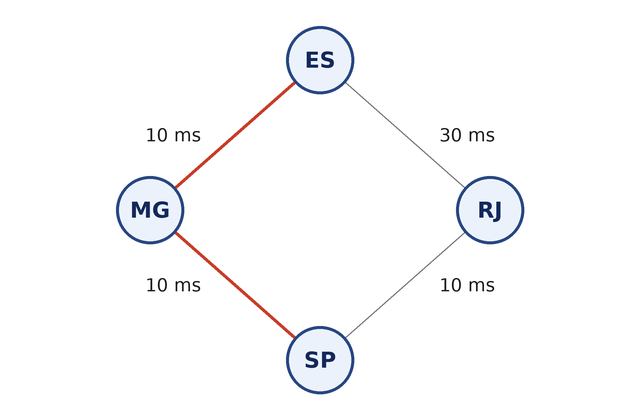
\includegraphics[width=0.55\textwidth]{../figures/diamond.png}
  \caption{The diamond instance. The minimum-cost path ES, MG, SP (cost 20) is drawn in red.}
  \label{fig:diamond}
\end{figure}

\paragraph{Dijkstra.} Table~\ref{tab:dijkstra-trace} shows the state after each iteration.

\begin{table}[htbp]
\centering
\begin{tabular}{clrrrrp{5.2cm}}
\toprule
Step & Visited & $d$[ES] & $d$[MG] & $d$[RJ] & $d$[SP] & Action \\
\midrule
0 & \{\} & 0 & $\infty$ & $\infty$ & $\infty$ & pick ES (smallest unvisited) \\
1 & \{ES\} & 0 & 10 & 30 & $\infty$ & relax ES's edges; pick MG (10) \\
2 & \{ES, MG\} & 0 & 10 & 30 & 20 & relax MG--SP ($10+10<\infty$); pick SP (20 < 30) \\
3 & \{ES, MG, SP\} & 0 & 10 & 30 & 20 & target reached, stop \\
\bottomrule
\end{tabular}
\caption{Dijkstra on the diamond, source ES, target SP.}
\label{tab:dijkstra-trace}
\end{table}

The result is ES, MG, SP at cost $20$ in $2$ hops. RJ is never improved below $30$, and the search stops
as soon as SP is selected, so RJ's distance is irrelevant to this query. The counters are $16$ comparisons
($3\times 4$ for the scans, plus $4$ edge checks) and $3$ relaxations.

\paragraph{Bellman--Ford.} The $8$ directed edges are relaxed per pass, with up to $|V|-1=3$ passes. Pass 1
gives $d=\{\text{ES}:0,\ \text{MG}:10,\ \text{RJ}:30,\ \text{SP}:20\}$ (the edge RJ to SP would offer $30+10=40$,
no improvement). Pass 2 improves nothing, so the loop stops after $2$ passes instead of $3$. The result is the
same path and the same cost, $20$, as it must be; the counters are $16$ comparisons ($2\times 8$) and $3$ relaxations.

\paragraph{BFS.} From ES, both MG and RJ are one hop away and SP is two hops away through either; MG was enqueued
first, so SP is discovered through it. The result is again ES, MG, SP at cost $20$, with $6$ comparisons and no relaxations.
Here BFS agrees with the other two \emph{by coincidence}: the fewest-hop path happens to also be the cheapest. That is exactly why
the report also needs instances where they diverge, Sections~\ref{sec:rnp} and \ref{sec:live}; a synthetic one is the
test graph in which A--B--D costs $140$ in $2$ hops while A--C--X--D costs $15$ in $3$ hops.

\subsection{Test instance 2: the real 27-node RNP backbone}
\label{sec:rnp}

The second instance is the real RNP backbone, the Brazilian research network the testbed is modeled on:
$27$ nodes (one PoP per state or region) and $44$ undirected links. The edge weight is the real measured
round-trip time in milliseconds. (An earlier draft of the code had no delay data and used $1/\text{capacity}$ as
a proxy; that mode is kept only for comparison and is not the recommended cost.) Two queries were run, and
Table~\ref{tab:rnp} summarizes them.

\begin{table}[htbp]
\centering
\begin{tabular}{llrrrrr}
\toprule
Query & Algorithm & Hops & Cost (ms) & Comparisons & Relaxations & Result \\
\midrule
ES $\to$ AC & Dijkstra & 5 & 66.42 & 787 & 44 & optimal \\
 & Bellman--Ford & 5 & 66.42 & 440 & 48 & optimal \\
 & BFS & 5 & 66.42 & 86 & 0 & same path \\
\midrule
RJ $\to$ RR & Dijkstra & 4 & 98.15 & 815 & 44 & optimal \\
 & Bellman--Ford & 4 & 98.15 & 440 & 38 & optimal \\
 & BFS & 3 & 144.01 & 70 & 0 & +47\% cost \\
\bottomrule
\end{tabular}
\caption{The three algorithms on the real RNP backbone (cost = measured RTT).}
\label{tab:rnp}
\end{table}

\paragraph{ES $\to$ AC (Espírito Santo to Acre).} Opposite corners of the country. All three algorithms agree:
ES, BA, DF, MT, RO, AC, five hops, $66.42$~ms. On this pair, minimizing hops also minimizes latency. It is
reported precisely \emph{because} it does not diverge: not every pair should, and a report showing only
diverging examples would be cherry-picking.

\paragraph{RJ $\to$ RR (Rio de Janeiro to Roraima).} Here they genuinely disagree, on real measured data and
not on a textbook example. BFS takes RJ, SP, CE, RR: three hops, but $144.01$~ms. Dijkstra and Bellman--Ford
take RJ, MG, DF, AM, RR: four hops, $98.15$~ms. The path with fewer hops is $47\%$ \emph{slower}. Dijkstra and
Bellman--Ford agree exactly, as the oracle requires.

\subsection{Execution time and scaling}
\label{sec:scaling}

On $4$ or even $27$ nodes every algorithm finishes in microseconds and the measured time is mostly Python call
overhead. To expose the asymptotic behaviour the experiment runs all three on random connected graphs of growing
size (average degree $3$, fixed seed), $|V|\in\{10,20,30,50,100,200,500\}$, from the first to the last node in
sorted order. Table~\ref{tab:scaling} gives the operation counts and times for the largest sizes; the full data
is in \texttt{data/scaling.csv}, and Figures~\ref{fig:comparisons} and \ref{fig:time} plot all sizes on a
logarithmic vertical axis.

\begin{table}[htbp]
\centering
\begin{tabular}{rrrrrrrr}
\toprule
 & & \multicolumn{3}{c}{Comparisons} & \multicolumn{3}{c}{Time ($\mu$s)} \\
$|V|$ & $|E|$ & Dijkstra & B--F & BFS & Dijkstra & B--F & BFS \\
\midrule
50 & 75 & 2125 & 600 & 101 & 78 & 36 & 8 \\
100 & 150 & 10299 & 1200 & 298 & 336 & 75 & 20 \\
200 & 300 & 32301 & 3600 & 533 & 958 & 217 & 37 \\
500 & 750 & 208341 & 9000 & 1385 & 5862 & 562 & 97 \\
\bottomrule
\end{tabular}
\caption{Operation counts and wall-clock time on random graphs (one run per size; timings are indicative).}
\label{tab:scaling}
\end{table}

\begin{figure}[htbp]
  \centering
  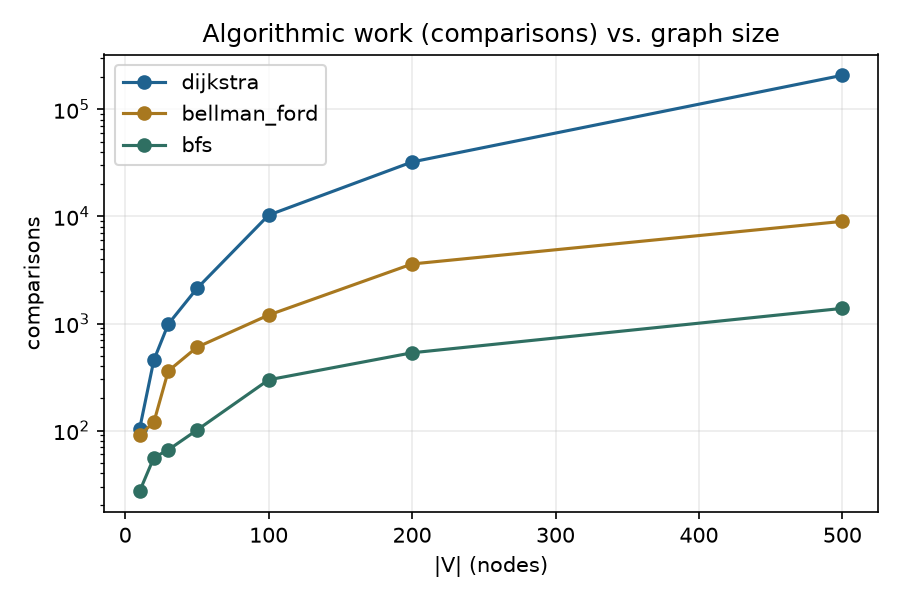
\includegraphics[width=0.8\textwidth]{../figures/comparisons_vs_n.png}
  \caption{Algorithmic work (comparisons) versus graph size, logarithmic vertical axis.}
  \label{fig:comparisons}
\end{figure}

\begin{figure}[htbp]
  \centering
  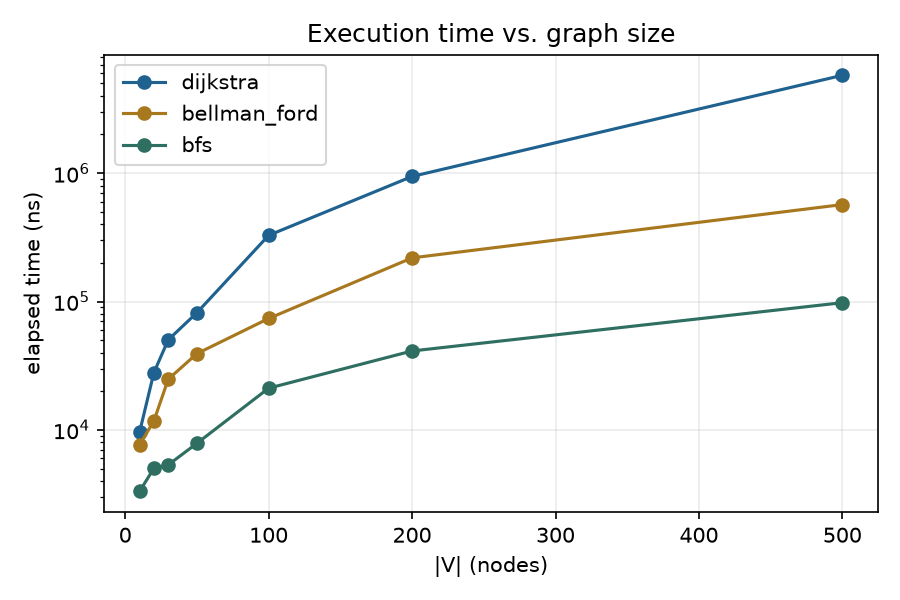
\includegraphics[width=0.8\textwidth]{../figures/time_vs_n.png}
  \caption{Execution time versus graph size, logarithmic vertical axis.}
  \label{fig:time}
\end{figure}

\paragraph{What the data shows.}
Dijkstra's work grows roughly quadratically: from $|V|=100$ to $500$, a factor of $5$ in size, comparisons grow by
a factor of $20$ (not the full $25$, because the search stops once the target is settled). Bellman--Ford grows by
$7.5$, consistent with $\Theta(kE)$: $E$ grows by $5$ while the number of passes $k$ stays small ($2$ to $6$ over all sizes), since
these random graphs have a short shortest-path tree. BFS grows by $4.6$, linear in $V+E$.

\paragraph{An honest surprise.}
On these sparse random graphs the array-based Dijkstra is \emph{slower} than Bellman--Ford, by a factor of about $10$
at $|V|=500$, although Bellman--Ford has the worse worst-case bound, $\Theta(VE)$ against $\Theta(V^2)$. The reason is
that the bound is only a worst case: early termination makes Bellman--Ford do about $kE$ work with a small $k$, while
the array version of Dijkstra pays a full $\Theta(V)$ scan in every iteration regardless of graph shape. This is the
difference between asymptotic class and the instance actually run, and it is the argument for the heap-based
variant ($O((V+E)\log V)$), which we did not implement. Two limits apply to every number here: each size was run once
with a fixed seed, and times are in an interpreted language. The operation counts are the more trustworthy evidence.

\paragraph{Divergence of BFS.}
The same runs show BFS finding a costlier path on four of the seven graphs ($|V|=20,30,50,200$). At $|V|=30$ it
returns a $3$-hop path of cost $94.73$ where Dijkstra finds a $5$-hop path of cost $75.0$.

\subsection{Correctness oracle and tests}
\label{sec:oracle}

Because Dijkstra and Bellman--Ford solve the same problem, \texttt{check\_correctness} compares their costs after every
run and raises an error on any mismatch. We treat this as a result in its own right and not only a testing detail:
it is evidence that two independently written implementations, based on different paradigms, are correct
\emph{relative to each other}. It held on the diamond, on the RNP backbone, on random graphs, and on live data
(next section). The unit-test suite (17 tests, all passing) covers the graph structure, the shared contract run
against all three classes, the diverging case, the agreement of Dijkstra and Bellman--Ford, the topology loaders,
and the live-API loader.

\subsection{Validation on a live testbed}
\label{sec:live}

The static data files could in principle disagree with what actually runs. A loader builds the graph directly from the
REIN console's \texttt{GET /api/testbed}, which describes the real running topology, pulled while an \texttt{rnp}
experiment was up (deployer and supervisor live). The algorithms needed \textbf{zero changes}; only a new loader
was added, which is the purpose of keeping the graph's surface to \texttt{add\_edge} and \texttt{neighbors}.
For BA to RJ, on the live graph ($|V|=27$, $|E|=44$):

\begin{lstlisting}[language={}, caption={Live-graph query BA to RJ (live testbed, RNP experiment).}, label={lst:live}]
dijkstra      hops=2 cost=14.430 path=BA -> MG -> RJ
bellman_ford  hops=2 cost=14.430 path=BA -> MG -> RJ
bfs           hops=2 cost=35.000 path=BA -> ES -> RJ
correctness oracle (dijkstra == bellman_ford): True
\end{lstlisting}

Two findings. First, the oracle holds on live data and not only on files. Second, this divergence is subtler than
RJ $\to$ RR: BFS and the other two pick paths with the \emph{same} hop count ($2$) but a cost ratio of $2.4$
($35.0$ against $14.43$~ms). BFS does not fail by taking more hops; it fails by breaking a hop-count \emph{tie}
arbitrarily, on insertion order, with no way to know that one of the tied options is far cheaper. This is arguably a
better illustration than ``more hops is worse'': even when hop count ties, it says nothing about which tied path to prefer.

One unit catch, documented so that the two loaders are not mistaken for disagreeing. The console's live delay is a
\emph{one-way} per-direction value (what is handed to \texttt{tc netem} for each direction of a link), while the static
\texttt{RTT\_MATRIX} is a \emph{round-trip} time. For the link AC--RO the static file gives $7.02$~ms and the live value is
$3.51$~ms, exactly half. Each is internally consistent; they are simply different units.

% ---------------------------------------------------------------------------
\section{Does it matter beyond the assignment?}
\label{sec:relevance}

\paragraph{An open issue asks for exactly this.}
Issue \texttt{lft\#10} of the project (``Função de Cálculo do melhor Caminho'', opened 2025-11-23, still open) asks for a function
that, given the topology matrix and the sets of client and server nodes, returns an ordered list of nodes or links for the
optimal client-to-server path, deterministically. That is almost exactly the contract of \texttt{PathFinder.find\_path()}.

\paragraph{It is already implemented, with heavier machinery.}
The platform's routine \texttt{cdn\_qoe.py::solve\_shortest\_path\_with\_constraints()} already does this for the
\texttt{cdn-qoe} intent. It scrapes ONOS's CLI with regular expressions to build the topology and then formulates the path as a
min-cost-flow integer linear program (one binary variable per edge, flow conservation), solved once per candidate target server by
OR-Tools with the SCIP backend.

\paragraph{The ILP is solving plain shortest path.}
The objective's only per-\emph{edge} term is $a\cdot\text{RTT}[i][j]$. The throughput term $b\cdot tx$ is a single offset per
\emph{target}: it never influences which edges are chosen, only the comparison between candidate servers after each shortest path is
found. So for a fixed target the program reduces to
\emph{minimize the sum of RTT along the path from source to target}, which is textbook weighted shortest path.
Dijkstra solves the identical problem on the identical graph with an identical optimum, in polynomial time, with no external
solver, and returns an inspectable path instead of a solver certificate. The loop over candidate servers need not change;
only its inner solve would.

\paragraph{Mapping to what already runs.}
Each algorithm here corresponds to something real in the stack (Table~\ref{tab:mapping}).

\begin{table}[htbp]
\centering
\begin{tabular}{lp{9.5cm}}
\toprule
Algorithm & Corresponds to \\
\midrule
BFS & ONOS's default hop-count path service, used by the deployer's middlebox chaining and by the \texttt{fwd} mode \\
Dijkstra & what the \texttt{ospf} mode already does (RFC 2328 \cite{rfc2328}), and what the \texttt{cdn\_qoe.py} ILP is provably equivalent to, per target \\
Bellman--Ford & the required literature comparison; not currently used in REIN \\
\bottomrule
\end{tabular}
\caption{Where each algorithm appears in the existing stack.}
\label{tab:mapping}
\end{table}

\paragraph{Caveats, stated plainly.}
The equivalence holds for the code \emph{as it stands}: one client's flow at a time, no shared link-capacity constraint across
simultaneous clients. Also, building the cost matrix by scraping CLI text with regular expressions is fragile; a previous
author already patched a case in which a fractional latency such as \texttt{4.38ms} failed an integer-only pattern and the link
silently kept a cost of zero, so the solver treated it as a free hop. A typed REST call would not have this failure mode.
Turning this into a real change to the platform needs a live ONOS-REST topology loader, the multi-target wrapper, and
agreement from the owner of \texttt{cdn\_qoe.py} on the question that follows.

% ---------------------------------------------------------------------------
\section{Advanced scenario: when shortest path stops being the right model}
\label{sec:nphard}

The single-commodity reduction holds only because today's deployer routes one client's request at a time. When several clients
must be routed \emph{together} over links of finite capacity, the problem changes class. This section states precisely why, and
it is presented separately from the main comparison because the remedy is not ``turn the ILP back on''.

\paragraph{What changes with a second client.}
Every link has a finite capacity. If two clients' paths share a link, their combined demand must not exceed it. Given several
(source, target, demand) triples, called \emph{commodities}, assign each a path so that no capacity is exceeded, at minimum total cost:
this is the \emph{multi-commodity flow} problem. A resource shared \emph{across} otherwise independent subproblems turns ``two easy
problems'' into ``one hard problem'', a pattern as old as job-shop scheduling and bin packing.

\paragraph{Why independent Dijkstra breaks.}
Dijkstra has no notion of remaining capacity or of a second flow. Route ten similar clients independently and all ten receive
the identical cheapest path, saturating one link while parallel links sit idle. Routing the clients \emph{sequentially} (give the first its best
path, subtract its usage, route the second on what is left) does not fix this either: the first client gets its true optimum and may
consume a bottleneck that a later client needs, forcing a detour it would have avoided had the first been routed slightly worse. The
\emph{order of arrival} silently determines the outcome, which a research testbed should not depend on.

\paragraph{The fork in the road: can traffic be split?}
This is where the complexity class is decided, and the two cases are not ``equally hard with a bigger solver''.
\begin{itemize}
  \item \textbf{Splittable} (a client's traffic may be divided over several paths). Flow conservation and capacity constraints are
        linear, the objective is linear, and the variables are continuous flow amounts. This is a \emph{linear program}, solvable in
        polynomial time (Khachiyan \cite{khachiyan1979}; interior-point and simplex-family methods in practice). Splittable
        multi-commodity flow with a thousand clients is still polynomial.
  \item \textbf{Unsplittable} (each client's traffic travels as one undivided path, which is what the issue asks for: ``an ordered list of
        nodes or links''). The variables become $0/1$ (is this edge on this client's path?), the feasible region is no longer a convex shape a
        linear-programming solver can walk, and the choice is one path per client among exponentially many, under a constraint coupling every
        client's choice to every other's. This is \emph{integer} linear programming, and this case is a named result: Even, Itai and
        Shamir \cite{even1976} proved that the integral two-commodity flow problem is \textbf{NP-complete}, in both the directed and
        undirected case, with as few as \textbf{two} commodities.
\end{itemize}
So the precise answer to ``why does this need ILP'' is that \emph{the no-splitting requirement combined with a shared capacity constraint}
creates the hardness, not simply ``more than one client''. Splittable with a thousand clients is polynomial; unsplittable with two is already
NP-complete.

\paragraph{Why Dijkstra specifically cannot be patched.}
Dijkstra's proof (Section~\ref{sec:technique}) rests on one guarantee: once a node is selected with its final distance, that distance can never
improve, \emph{because every edge weight is a fixed number, known in advance, that does not depend on any other decision being made}. The moment a
second client competes for the same link, an edge's usability for the first depends on whether the second's not-yet-decided path also wants
it. The edge's effective cost is no longer an input of the algorithm but an output of the very decision being made, for a different commodity.
Nothing can be bolted onto Dijkstra's loop to account for that, because its mechanism assumes the quantity it optimizes over does not move
while it runs. This is also why running Dijkstra once per client does not help (the ``sequential trap'' above): each call privately assumes
its weights are final, when the previous client's choice has silently consumed capacity the next call cannot see.

\paragraph{Why use ILP anyway, if it is NP-hard?}
Because NP-hardness describes the worst case, not every instance. Modern solvers (OR-Tools/SCIP, CPLEX, Gurobi) use branch and bound:
solve the easy linear relaxation for a bound, then explore only branches that could beat it. On realistic sizes (a handful of
concurrent clients, a few dozen PoPs) this typically finds the exact optimum quickly, so reaching for OR-Tools is the correct tool for the multi-client
problem. It is only overkill for the version the code solves \emph{today}.

\paragraph{The broader lesson.}
A problem need not look complicated to be NP-hard: it only has to stop being decomposable into independent pieces. One shortest path is
easy because nothing else depends on the choice. Add a shared finite resource that several such choices must divide, and the problem can change
complexity class with no other change, not because the sub-problems got harder, but because they stopped being separable.

\paragraph{Consequence for the design.}
Joint routing does not become a fourth \texttt{PathFinder}: its signature is not \texttt{find\_path(graph, source, target)}. It needs every
active client's request and per-edge capacities at once, and it returns a \emph{set} of paths. Forcing it into the hierarchy would
either require more than the interface promises its callers or return something different, which is precisely the substitutability
violation the contract forbids. The honest design is a second interface one level up: a sequential allocator that calls \texttt{PathFinder}
once per client (today's uncoordinated behaviour, made explicit) alongside an ILP allocator that extends the existing formulation with
$\sum \text{flow}(i,j)\le \text{capacity}(i,j)$ constraints, with the deployer's policy choosing between them. That choice belongs to the owner of
\texttt{cdn\_qoe.py}; it is future work and nothing built here changes.

% ---------------------------------------------------------------------------
\section{Decisions and limitations}
\label{sec:decisions}

\begin{itemize}
  \item \textbf{Non-negative weights only.} Every cost used (delay in ms, inverse capacity) is non-negative. Bellman--Ford can in principle
        handle negative weights; the implementation does not detect negative cycles, since none can occur here.
  \item \textbf{Undirected links.} Each link is stored in both directions with the same weight.
  \item \textbf{Standalone package.} The implementation reads the topology data but imports nothing from the testbed (no Docker, no ONOS),
        so it runs anywhere with Python and no external libraries. All three algorithms are written from scratch, with no graph library.
  \item \textbf{Heap-free Dijkstra.} Chosen for a clean $\Theta(V^2)$ analysis; its consequence for speed on sparse graphs is discussed in
        Section~\ref{sec:scaling}.
  \item \textbf{Single runs.} Timing results come from one run per size with a fixed seed, so they are indicative; the operation counters are exact.
\end{itemize}

% ---------------------------------------------------------------------------
\section{Members}
\label{sec:members}

This work was developed individually by Danrley Pereira, who wrote the algorithms, the experiment code, the tests, the analysis and this report.

% ---------------------------------------------------------------------------
\section{Conclusion}
\label{sec:conclusion}

Dijkstra and Bellman--Ford, implemented behind one contract, agreed on the optimal cost on every instance tried: the diamond, the real
27-node RNP backbone, random graphs up to $500$ nodes, and a live testbed. That agreement served as a correctness oracle across two different
design paradigms. Hop-count search disagreed on real data, once by $47\%$ in cost, and once, on the live graph, by breaking a tie between
equal-hop paths without any knowledge of their cost. The complexity analysis of the code as written, not of a textbook version, gave
$\Theta(V)$, $\Theta(V^2)$ and $\Theta(V^2)$ for Dijkstra's best, worst and average case, and the measurements confirmed the quadratic growth.

The main difficulties were of three kinds. First, complexity analysis must follow the implementation: the best case of Dijkstra was first written down
as $\Theta(V^2)$ and was corrected to $\Theta(V)$ only by checking it against the code; this is why the assignment asks for the complexity of
\emph{your implementation}. Second, the asymptotically better algorithm was not the faster one on the instances run: array-based Dijkstra lost to
Bellman--Ford with early termination on sparse graphs, a reminder that a worst-case bound is not a prediction. Third, fitting the problem to the
real system showed that the correct tool depends on the shape of the problem: for one client at a time the existing integer program is plain
shortest path and Dijkstra suffices, while the moment clients share capacity and cannot be split, the problem is NP-hard and an ILP is the right
answer.

\bibliographystyle{plain}
\bibliography{refs}

\end{document}
